%!TEX root = DisenoProyecto_LuisGomez.tex
%%!TEX root = DisenoProyecto_LuisGomez.tex
%%!TEX root = DisenoProyecto_LuisGomez.tex
%%!TEX root = DisenoProyecto_LuisGomez.tex
%\input{10_Diagrama_Actividades.tex}

%\begin{consigna}{red}
%Armar el AoN a partir del WBS definido en la etapa anterior. 
%
%%La figura \ref{fig:AoN} fue elaborada con el paquete latex tikz y pueden consultar la siguiente referencia \textit{online}:
%
%%\url{https://www.overleaf.com/learn/latex/LaTeX_Graphics_using_TikZ:_A_Tutorial_for_Beginners_(Part_3)\%E2\%80\%94Creating_Flowcharts}
%
%\end{consigna}

%\begin{figure}[htpb]
%\centering 
%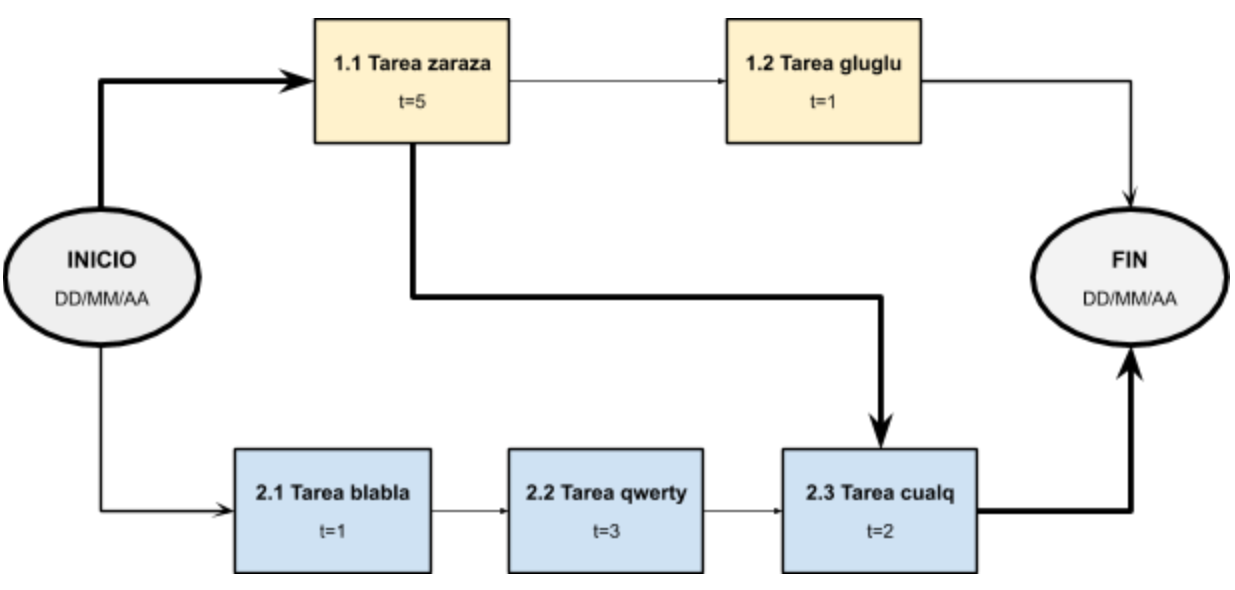
\includegraphics[width=.8\textwidth]{./Figuras/AoN.png}
%\caption{Diagrama de \textit{Activity on Node}.}
%\label{fig:AoN}
%\end{figure}
%
%Indicar claramente en qué unidades están expresados los tiempos.
%De ser necesario indicar los caminos semicríticos y analizar sus tiempos mediante un cuadro.
%Es recomendable usar colores y un cuadro indicativo describiendo qué representa cada color, como se muestra en el siguiente ejemplo:

El diagrama de flujo de la figura \ref{fig:diagrama}, se presenta una estructura general para la ejecución del proyecto de tesis. Comenzando con la gestión del proyecto, el esquema traza una ruta cronológica que incluye diseño, construcción de hardware y programación de firmware, los cuales ocurren de manera concurrente. Estas fases convergen en una etapa de pruebas, seguida de ajustes finales y la generación de documentación académica. Finalmente, el proyecto culmina con la entrega del trabajo final. Notar que cada una de las celdas contiene el tiempo estimado de las actividades y el tiempo acumulado general, con el formato:  \textbf{\textit{``tiempo bloque actividades''  / ``tiempo total acumulado"}} en horas.


\begin{figure}[!hbp]
	
	\centering
	\begin{tikzpicture}[node distance=2.2cm]
	
	\tikzstyle{block} = [rectangle, draw, fill=blue!10, text width=6em, text centered, rounded corners, minimum height=3em]
	\tikzstyle{line} = [draw, -latex']
	\tikzstyle{circleblock} = [circle, draw, fill=red!10, text centered, minimum size=3em]
	
	\node [circleblock] (init) {Inicio (0 hs)};
	\node [block, below of=init]              	(1) {1. Gestión (100/100 hs)};
	\node [block, below of=1]                  	(2) {2. Diseño (60/160 hs)};
	\node [block, left of=2, node distance=3cm]	(3) {3. Hardware (120/280 hs)};
	\node [block, right of=2, node distance=3cm](4) {4. Firmware (110/280 hs)};
	\node [block, below of=2]                  	(5) {5. Pruebas (80/360 hs)};
	\node [block, below of=5]                  	(6) {6. Ajustes (40/400 hs)};
	\node [block, below of=6]                 	(7) {7. Escritos (180/580 hs)};
	\node [block, below of=7] 					(8) {8. Entrega (40/620 hs)};
	\node [circleblock, below of=8]             (fin) {Fin (620 hs)};
	
	\path [line] (init) -- 	(1);
	\path [line] (1) 	-- 	(2);
	\path [line] (2) 	-- 	(3);
	\path [line] (2) 	-- 	(4);
	\path [line] (4) 	|- 	(5);
	\path [line] (3) 	|- 	(5);
	\path [line] (5) 	-- 	(6);
	\path [line] (6) 	-- 	(7);
	\path [line] (7) 	-- 	(8);
	\path [line] (8) 	-- 	(fin);
	
	
	\end{tikzpicture}
	\caption{Diagrama de flujo para la gestión del proyecto}
	\label{fig:diagrama}
\end{figure}






%\begin{consigna}{red}
%Armar el AoN a partir del WBS definido en la etapa anterior. 
%
%%La figura \ref{fig:AoN} fue elaborada con el paquete latex tikz y pueden consultar la siguiente referencia \textit{online}:
%
%%\url{https://www.overleaf.com/learn/latex/LaTeX_Graphics_using_TikZ:_A_Tutorial_for_Beginners_(Part_3)\%E2\%80\%94Creating_Flowcharts}
%
%\end{consigna}

%\begin{figure}[htpb]
%\centering 
%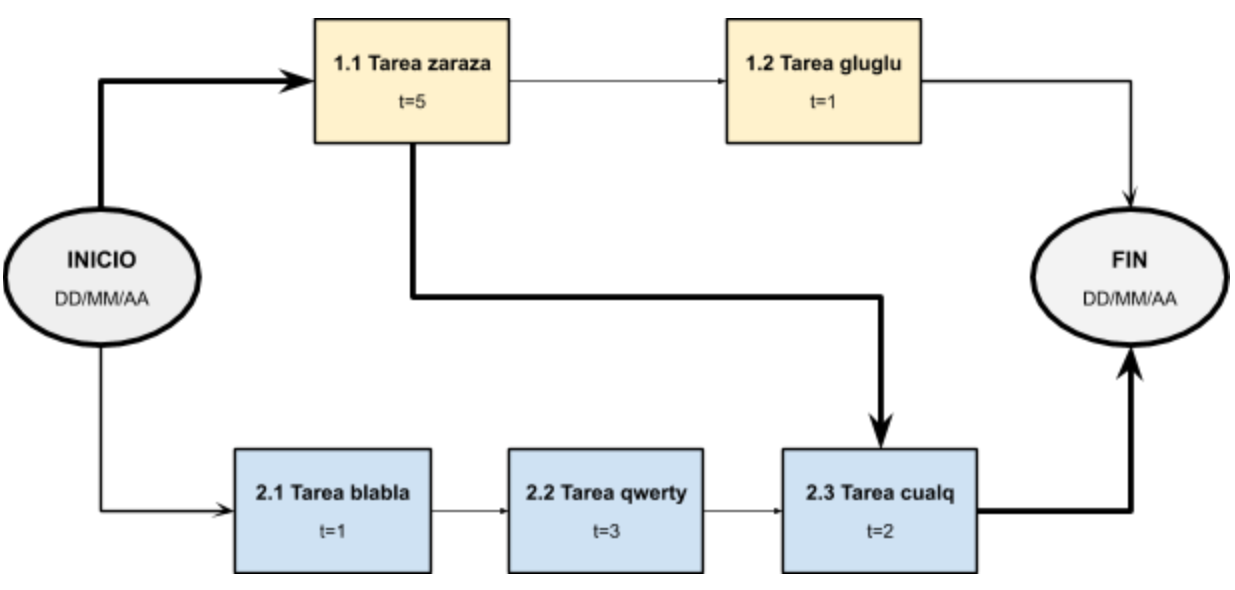
\includegraphics[width=.8\textwidth]{./Figuras/AoN.png}
%\caption{Diagrama de \textit{Activity on Node}.}
%\label{fig:AoN}
%\end{figure}
%
%Indicar claramente en qué unidades están expresados los tiempos.
%De ser necesario indicar los caminos semicríticos y analizar sus tiempos mediante un cuadro.
%Es recomendable usar colores y un cuadro indicativo describiendo qué representa cada color, como se muestra en el siguiente ejemplo:

El diagrama de flujo de la figura \ref{fig:diagrama}, se presenta una estructura general para la ejecución del proyecto de tesis. Comenzando con la gestión del proyecto, el esquema traza una ruta cronológica que incluye diseño, construcción de hardware y programación de firmware, los cuales ocurren de manera concurrente. Estas fases convergen en una etapa de pruebas, seguida de ajustes finales y la generación de documentación académica. Finalmente, el proyecto culmina con la entrega del trabajo final. Notar que cada una de las celdas contiene el tiempo estimado de las actividades y el tiempo acumulado general, con el formato:  \textbf{\textit{``tiempo bloque actividades''  / ``tiempo total acumulado"}} en horas.


\begin{figure}[!hbp]
	
	\centering
	\begin{tikzpicture}[node distance=2.2cm]
	
	\tikzstyle{block} = [rectangle, draw, fill=blue!10, text width=6em, text centered, rounded corners, minimum height=3em]
	\tikzstyle{line} = [draw, -latex']
	\tikzstyle{circleblock} = [circle, draw, fill=red!10, text centered, minimum size=3em]
	
	\node [circleblock] (init) {Inicio (0 hs)};
	\node [block, below of=init]              	(1) {1. Gestión (100/100 hs)};
	\node [block, below of=1]                  	(2) {2. Diseño (60/160 hs)};
	\node [block, left of=2, node distance=3cm]	(3) {3. Hardware (120/280 hs)};
	\node [block, right of=2, node distance=3cm](4) {4. Firmware (110/280 hs)};
	\node [block, below of=2]                  	(5) {5. Pruebas (80/360 hs)};
	\node [block, below of=5]                  	(6) {6. Ajustes (40/400 hs)};
	\node [block, below of=6]                 	(7) {7. Escritos (180/580 hs)};
	\node [block, below of=7] 					(8) {8. Entrega (40/620 hs)};
	\node [circleblock, below of=8]             (fin) {Fin (620 hs)};
	
	\path [line] (init) -- 	(1);
	\path [line] (1) 	-- 	(2);
	\path [line] (2) 	-- 	(3);
	\path [line] (2) 	-- 	(4);
	\path [line] (4) 	|- 	(5);
	\path [line] (3) 	|- 	(5);
	\path [line] (5) 	-- 	(6);
	\path [line] (6) 	-- 	(7);
	\path [line] (7) 	-- 	(8);
	\path [line] (8) 	-- 	(fin);
	
	
	\end{tikzpicture}
	\caption{Diagrama de flujo para la gestión del proyecto}
	\label{fig:diagrama}
\end{figure}






%\begin{consigna}{red}
%Armar el AoN a partir del WBS definido en la etapa anterior. 
%
%%La figura \ref{fig:AoN} fue elaborada con el paquete latex tikz y pueden consultar la siguiente referencia \textit{online}:
%
%%\url{https://www.overleaf.com/learn/latex/LaTeX_Graphics_using_TikZ:_A_Tutorial_for_Beginners_(Part_3)\%E2\%80\%94Creating_Flowcharts}
%
%\end{consigna}

%\begin{figure}[htpb]
%\centering 
%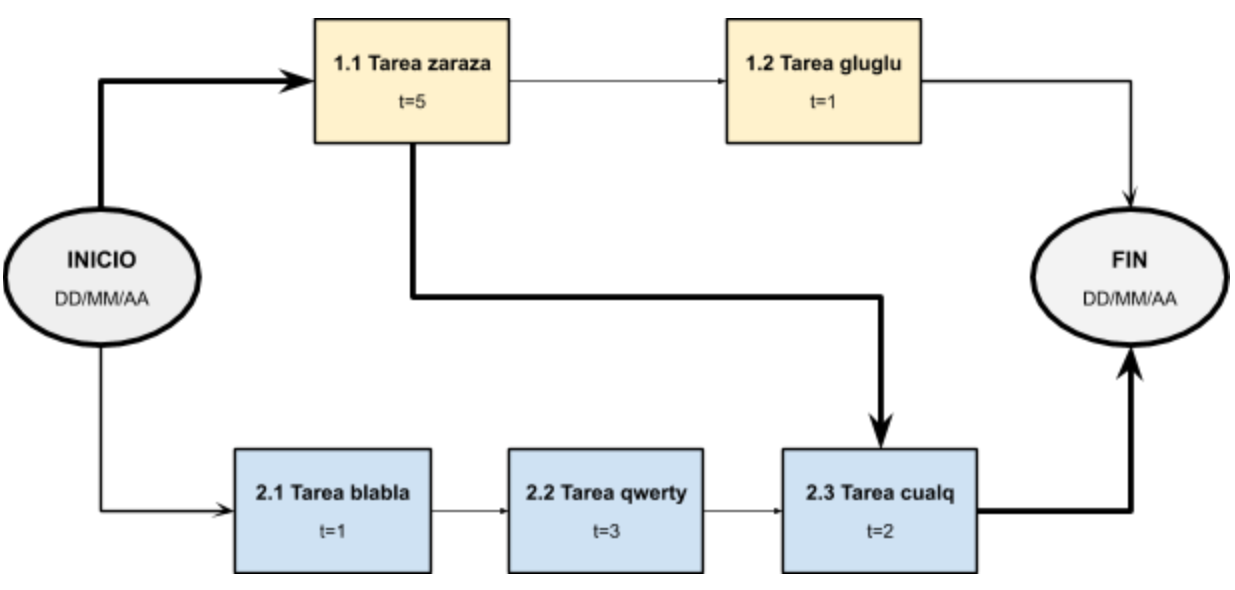
\includegraphics[width=.8\textwidth]{./Figuras/AoN.png}
%\caption{Diagrama de \textit{Activity on Node}.}
%\label{fig:AoN}
%\end{figure}
%
%Indicar claramente en qué unidades están expresados los tiempos.
%De ser necesario indicar los caminos semicríticos y analizar sus tiempos mediante un cuadro.
%Es recomendable usar colores y un cuadro indicativo describiendo qué representa cada color, como se muestra en el siguiente ejemplo:

El diagrama de flujo de la figura \ref{fig:diagrama}, se presenta una estructura general para la ejecución del proyecto de tesis. Comenzando con la gestión del proyecto, el esquema traza una ruta cronológica que incluye diseño, construcción de hardware y programación de firmware, los cuales ocurren de manera concurrente. Estas fases convergen en una etapa de pruebas, seguida de ajustes finales y la generación de documentación académica. Finalmente, el proyecto culmina con la entrega del trabajo final. Notar que cada una de las celdas contiene el tiempo estimado de las actividades y el tiempo acumulado general, con el formato:  \textbf{\textit{``tiempo bloque actividades''  / ``tiempo total acumulado"}} en horas.


\begin{figure}[!hbp]
	
	\centering
	\begin{tikzpicture}[node distance=2.2cm]
	
	\tikzstyle{block} = [rectangle, draw, fill=blue!10, text width=6em, text centered, rounded corners, minimum height=3em]
	\tikzstyle{line} = [draw, -latex']
	\tikzstyle{circleblock} = [circle, draw, fill=red!10, text centered, minimum size=3em]
	
	\node [circleblock] (init) {Inicio (0 hs)};
	\node [block, below of=init]              	(1) {1. Gestión (100/100 hs)};
	\node [block, below of=1]                  	(2) {2. Diseño (60/160 hs)};
	\node [block, left of=2, node distance=3cm]	(3) {3. Hardware (120/280 hs)};
	\node [block, right of=2, node distance=3cm](4) {4. Firmware (110/280 hs)};
	\node [block, below of=2]                  	(5) {5. Pruebas (80/360 hs)};
	\node [block, below of=5]                  	(6) {6. Ajustes (40/400 hs)};
	\node [block, below of=6]                 	(7) {7. Escritos (180/580 hs)};
	\node [block, below of=7] 					(8) {8. Entrega (40/620 hs)};
	\node [circleblock, below of=8]             (fin) {Fin (620 hs)};
	
	\path [line] (init) -- 	(1);
	\path [line] (1) 	-- 	(2);
	\path [line] (2) 	-- 	(3);
	\path [line] (2) 	-- 	(4);
	\path [line] (4) 	|- 	(5);
	\path [line] (3) 	|- 	(5);
	\path [line] (5) 	-- 	(6);
	\path [line] (6) 	-- 	(7);
	\path [line] (7) 	-- 	(8);
	\path [line] (8) 	-- 	(fin);
	
	
	\end{tikzpicture}
	\caption{Diagrama de flujo para la gestión del proyecto}
	\label{fig:diagrama}
\end{figure}






%\begin{consigna}{red}
%Armar el AoN a partir del WBS definido en la etapa anterior. 
%
%%La figura \ref{fig:AoN} fue elaborada con el paquete latex tikz y pueden consultar la siguiente referencia \textit{online}:
%
%%\url{https://www.overleaf.com/learn/latex/LaTeX_Graphics_using_TikZ:_A_Tutorial_for_Beginners_(Part_3)\%E2\%80\%94Creating_Flowcharts}
%
%\end{consigna}

%\begin{figure}[htpb]
%\centering 
%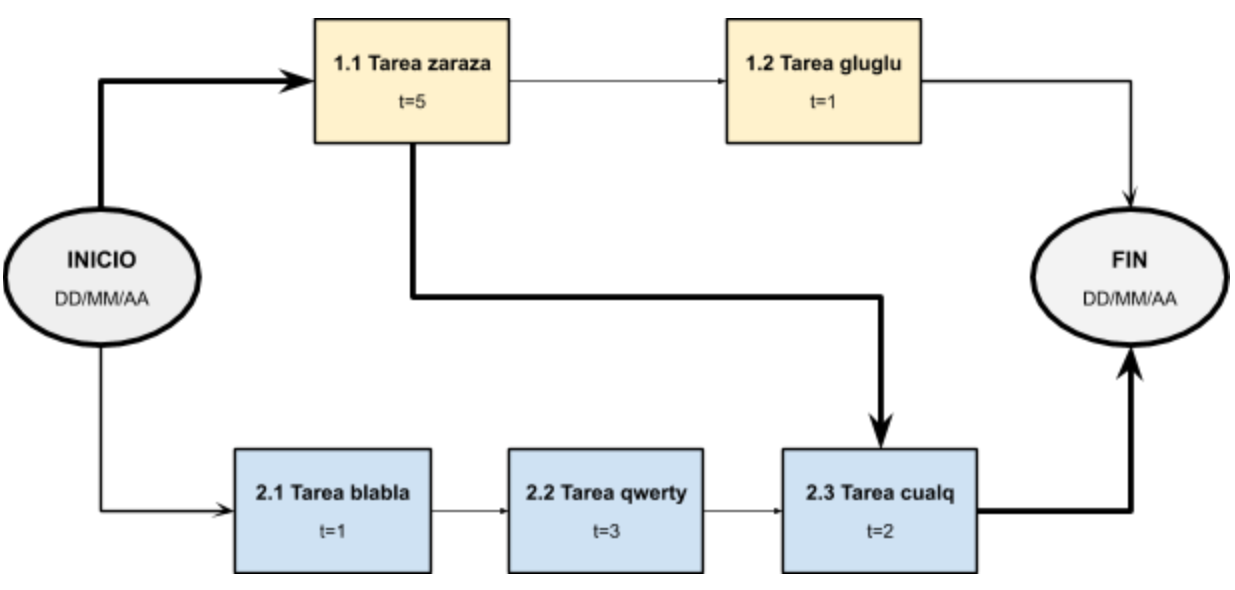
\includegraphics[width=.8\textwidth]{./Figuras/AoN.png}
%\caption{Diagrama de \textit{Activity on Node}.}
%\label{fig:AoN}
%\end{figure}
%
%Indicar claramente en qué unidades están expresados los tiempos.
%De ser necesario indicar los caminos semicríticos y analizar sus tiempos mediante un cuadro.
%Es recomendable usar colores y un cuadro indicativo describiendo qué representa cada color, como se muestra en el siguiente ejemplo:

En la figura \ref{fig:diagrama} se ilustra un diagrama de flujo que expone una estructura general para la ejecución del proyecto de tesis. Este proceso inicia con la gestión del proyecto y delinea una ruta cronológica que engloba el diseño, la construcción de hardware y la programación de firmware, aconteciendo estas de manera concurrente. Estas fases convergen en una etapa de pruebas, la cual es seguida por ajustes finales y la redacción de documentación académica. Finalmente, el proyecto concluye con la entrega del trabajo final. Es importante señalar que cada una de las celdas del diagrama de flujo especifican ``\textit{horas estimadas de cada actividades}" (HA), el ``\textit{camino crítico}" (CC) y los ``\textit{horas totales acumuladas}" (HT) desde el inicio del proyecto. Se presenta en el formato: \textbf{HA/{\color{red}CC}/HT} en días, indicado el la parte inferior de cada recuadro. Los tiempos y las flechas de color rojo ({\color{red}\faArrowDown})  muestran el camino crítico.



\begin{figure}[!hbp]
	\centering
	\begin{tikzpicture}[node distance=2.15cm]
	
	\tikzstyle{block} = [rectangle, draw, fill=blue!10, text width=7em, text centered, rounded corners, minimum height=3.5em]
	\tikzstyle{line} = [draw, -latex']
	\tikzstyle{critical_line} = [draw, red, very thick, -latex']
	\tikzstyle{circleblock} = [circle, draw, fill=red!10, text centered, minimum size=3em]
	
	\node [circleblock, align=center] (init) {Inicio \\22-08-2023};
	\node [block, below of=init] (1) {1. Gestión { 100/{\color{red}100}/100}};
	\node [block, below of=1] (2) {2. Diseño { 60/{\color{red}160}/160}};
	\node [block, left of=2, node distance=3cm, xshift=-1cm] (3) {3. Hardware { 120/{\color{red}280}/390}};
	\node [block, right of=2, node distance=3cm, xshift=1cm] (4) {4. Firmware 110/270/390};
	\node [block, below of=2] (5) {5. Pruebas { 80/{\color{red}360}/470}};
	\node [block, below of=5] (6) {6. Ajustes { 40/{\color{red}400}/510}};
	\node [block, below of=6] (7) {7. Escritos { 180/{\color{red}580}/690}};
	\node [block, below of=7] (8) {8. Entrega { 40/{\color{red}620}/730}};
	\node [circleblock, below of=8, align=center] (fin) {Fin \\22-05-2024}; % nodo actualizado
	
	\path [critical_line] (init) -- (1);
	\path [critical_line] (1) -- (2);
	\path [critical_line] (2) -- (3);
	\path [line] (2) -- (4);
	\path [line] (4) |- (5);
	\path [critical_line] (3) |- (5);
	\path [critical_line] (5) -- (6);
	\path [critical_line] (6) -- (7);
	\path [critical_line] (7) -- (8);
	\path [critical_line] (8) -- (fin);
	
	\end{tikzpicture}
	\caption{Diagrama de flujo para la gestión del proyecto.}
	\label{fig:diagrama}
\end{figure}






